\documentclass{article}
\usepackage{amsmath}
\usepackage{setspace}

\usepackage{graphicx}
\graphicspath{{images/}}
\usepackage{wrapfig}
\usepackage{comment}
\usepackage{listings}
\usepackage{xcolor}
\usepackage{float}
\usepackage[style=numeric]{biblatex}
\addbibresource{fish.bib}
\usepackage{comment}

\definecolor{codegreen}{rgb}{0,0.6,0}
\definecolor{codegray}{rgb}{0.5,0.5,0.5}
\definecolor{codepurple}{rgb}{0.58,0,0.82}
\definecolor{backcolour}{rgb}{0.95,0.95,0.92}
 
\lstdefinestyle{mystyle}{
    backgroundcolor=\color{backcolour},
    commentstyle=\color{codegreen},
    keywordstyle=\color{magenta},
    numberstyle=\tiny\color{codegray},
    stringstyle=\color{codepurple},
    basicstyle=\fontsize{10}{12}\ttfamily,
    breakatwhitespace=false,
    breaklines=true,
    %breaklines=false,
    captionpos=b,
    keepspaces=true,
    numbers=left,
    numbersep=5pt,
    showspaces=false,
    showstringspaces=false,
    showtabs=false,
    tabsize=2
}
 
\lstset{style=mystyle}

%\usepackage[letter,margin=1.5in]{geometry}
%\addtolength{\rightmargin}{-0.5in}
%\addtolength{\textwidth}{0.5in}
%\addtolength{\oddsidemargin}{-.875in}
%\addtolength{\evensidemargin}{-.875in}
%\addtolength{\textheight}{1.75in}

\makeatletter
\renewcommand\section{\clearpage\newpage\@startsection {section}{1}{\z@}%
	{-3.5ex \@plus -1ex \@minus -.2ex}%
	{2.3ex \@plus.2ex}%
	{\normalfont\Large\bfseries}}
\makeatother

\begin{document}

%==========================================================================
%==========================================================================
% Title pages.

\begin{comment}
\newcommand{\mytitle}{Report for End of Year on Progress on Fish Tracking Software}
\newcommand{\myauthor}{Ari Spraggins}

\newcommand{\myskip}{\vspace{0.5in}}
\newcommand{\layouttitle}[1]{{\bf\large\MakeUppercase{#1}}}
\setlength{\parindent}{0em}
\doublespace
\pagenumbering{roman}
\thispagestyle{empty}

\begin{center}

	\vspace{4in} 
	\layouttitle{\mytitle} \\ by \\ \myauthor
	
	\vspace{1in}
	A Thesis Submitted to the Faculty of \\
	The Wilkes Honors College \\
	in Partial Fulfillment of the Requirements for the Degree of \\
	Bachelor of Science in Liberal Arts and Sciences \\
	with a Concentration in Physics \\ 
	\vspace{1in} 
	Wilkes Honors College of \\
	Florida Atlantic University \\
	Jupiter, Florida \\
	May \number\year

\end{center}

\newpage

%==========================================================================

\vspace{4in}
\begin{center}
	\layouttitle{\mytitle} \\
	by \\
	\myauthor
\end{center}

\singlespace
\vspace{1in}
This thesis was prepared under the direction of the candidate's thesis advisor, Dr. Yaouen Fily, and has been approved by the members of their supervisory committee. It was submitted to the faculty of the Harriet L. Wilkes Honors College and was accepted in partial fulfillment of the requirements for the degree of Bachelor of Science in Liberal Arts and Sciences.

\vspace{1in}
SUPERVISORY COMMITTEE:

\newcommand{\myrule}{\vspace{0.5in}\rule{4in}{0.5pt} \\}

\myrule
Dr. Yaouen Fily 

\myrule 
{}[second reader]

\myrule
Interim Dean Timothy Steigenga, Harriet L. Wilkes Honors College 

\myrule
Date

\newpage

%==========================================================================

%\begin{center}
%	\layouttitle{Acknowledgements}
%\end{center}
\section*{Acknowledgements}
%\addcontentsline{toc}{section}{Acknowledgements}

\myskip
Some acknowledgements.

\newpage

%==========================================================================

%\begin{center}
%	\layouttitle{Abstract}
%\end{center}
\section*{Abstract}
\addcontentsline{toc}{section}{Abstract}

\myskip
\renewcommand{\arraystretch}{1.5}
\begin{tabular}{@{}l@{\hspace{3ex}}l}
	Author: & \myauthor \\
	Title: & \mytitle \\
	Institution: & Harriet L. Wilkes Honors College, Florida Atlantic University \\
	Thesis Advisor: & Dr. Yaouen Fily \\
	Degree: & Bachelor of Science in Liberal Arts and Sciences \\
	Concentration: & Physics \\
	Year: & \the\year
\end{tabular}

\myskip
\doublespace
\end{comment}
Automatic video tracking has had a major impact on animal behavior studies. One of the problems with using this to track the positions of animals has been keeping the animals distinct. To solve this problem for groups of fish, we will be using python code to track patterns of brightness as a visual identifier to track the fish using data from the labs of Dr. Keene, Dr. Duboue, and Dr. Kowalko, who all work with Mexican cavefish on the Jupiter campus.

\singlespace
\newpage

\begin{comment}
%==========================================================================

\tableofcontents

\listoftables

\listoffigures

\newpage

%==========================================================================
\end{comment}

\setlength{\parindent}{1em}
\pagenumbering{arabic}

%==========================================================================
%==========================================================================
% Thesis proper.


\section{Introduction}

\subsection{Tracking Animal Behaviour}
While visually pleasing, schooling is a rather challenging topic that has long befuddled animal scientists, due to the fact that to preform proper analysis of the animals' behavior, a vast quantity of positional data is needed. This has been alleviated recently with advances in technology, since scientists can now use computers to track the animals' positions. While this technically was possible before, this would require a person sitting in front of a video manually tracking the positions of each of the animals in question, which is what the program that we are writing aims to eliminate.

%talk about how interested in how schooling came to be? Schooling dynamics of related groups can provide insight in to how groups evolved. Now talk about trilab studying species that has variants that both do and don't school that are similar.
In particular, the group that this paper gets it's data from is looking at Mexican Tetra (\textit{latin name}) \cite{fishPaper}. One of the quirks of Mexican Tetra is that different groups have startling evolutionary differences such as one of the groups having not evolved schooling, despite being nominally the same species as the ones that did. However, one issue that arises is that it is impractical to quantify fish behavior without automated tracking. As such, this project aims to provide a program that tracks the fish so that the labs can analyse them.

Since fish motion has become so much easier to work with, some groups that were studying the fish are using this opportunity to study the lives and motion of different types of fish in much more detail and with much more data than they were before. One of these is an association of groups out of Jupiter, which are working on Mexican Tetra. These labs, headed by Dr. Keene, Dr. Duboue, and Dr. Kowalko, collectively known as the cavefish trilab, are currently interested in the evolution of behavior of Mexican Tetra, which necessitates a lot of video of the fish. Over the last few years the cavefish trilab has been collaborating with Dr. Fily, to apply physics techniques of collective grouping \cite{patch_kinematic_2020}. He has developed a software to track the fish, which is currently in use by the labs, but has the issue with maintaining the identities of the fish throughout the experiment, so this project aims to fix that. Since the trilab is working with video of Tetra, this presented an opportunity to apply these techniques to clean up the video they have produced. 

\subsection{Nature of the problem}

Before discussing how to maintain the identity of the fish as we track them, we must first talk a little about how the software locates them. The process starts by picking out the dark spots in the video caused by the contrast between the fish and the light background of the tank. The software then interprets each dark spot as a fish.

\begin{figure}[H]
	\centering
	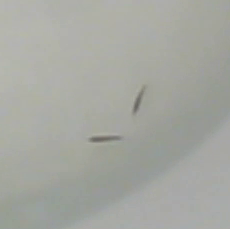
\includegraphics[width=.5\linewidth]{140cropped}
	\caption{The two fishes}
	\label{fig:fish}
\end{figure}

While this works well for determining the positions of objects at any given moment, it needs some extra work to be able to keep the fish straight, since there is no continuity.

\begin{figure}[H]
	\centering
	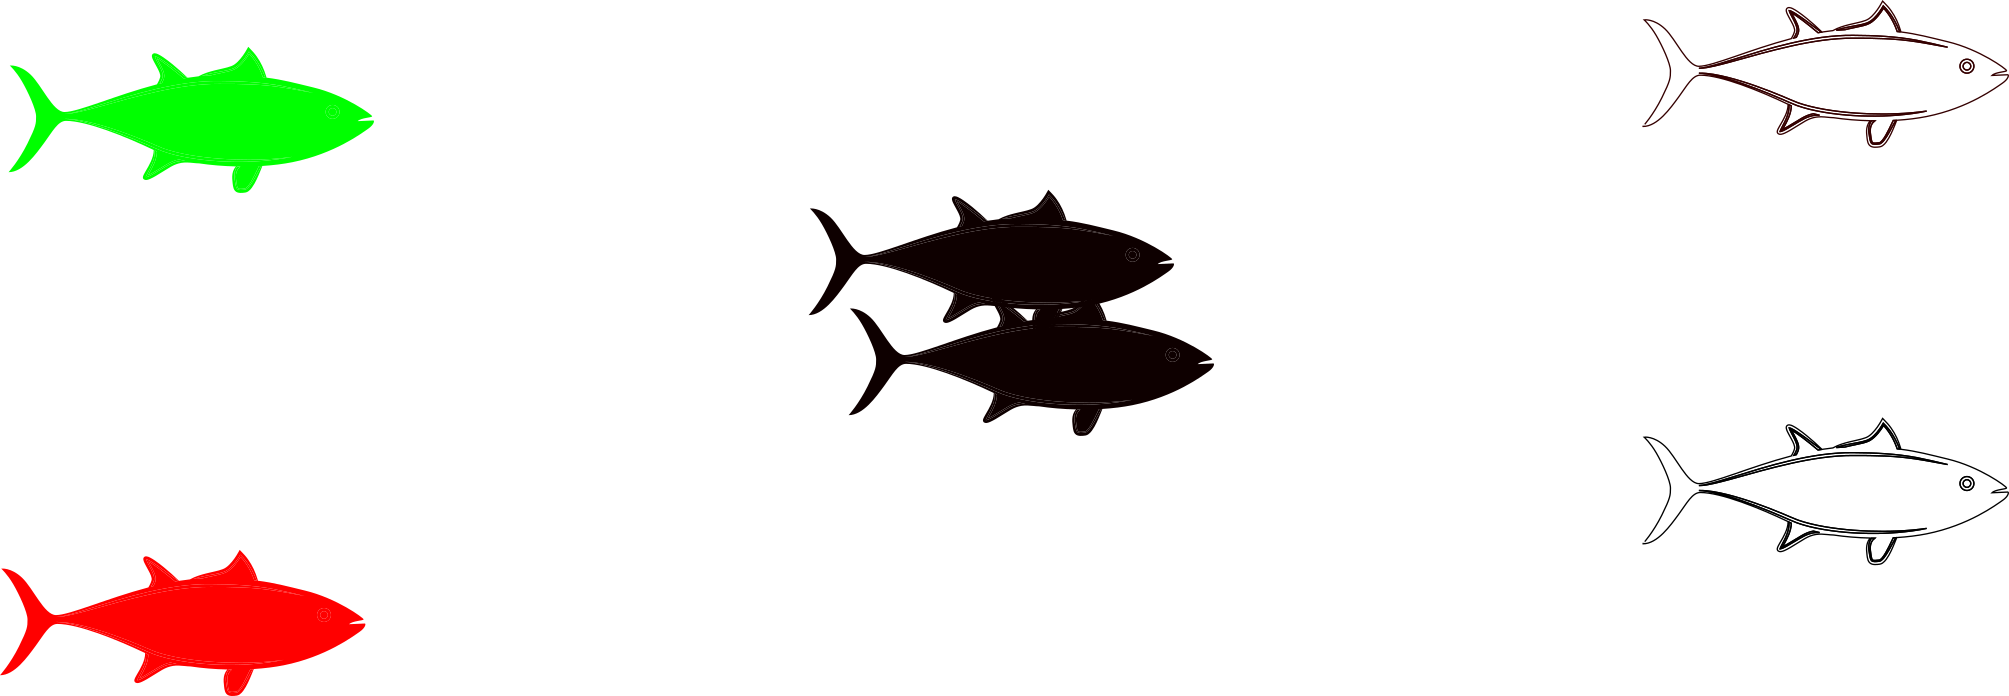
\includegraphics[width=\linewidth]{g1225}
	\caption{The program doesn't respect continuity}
	\label{fig:continuity}
\end{figure}

To do this we can compare how the fish have moved by tracking their positions relative to their last known positions on a frame by frame basis.

\begin{figure}[H]
	\centering
	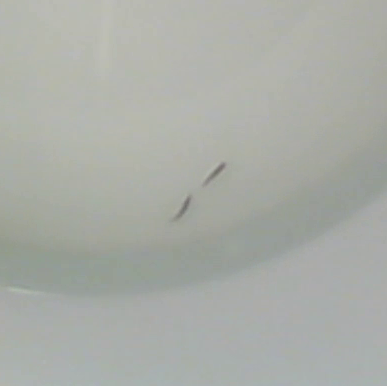
\includegraphics[width=.32\linewidth]{5133}
	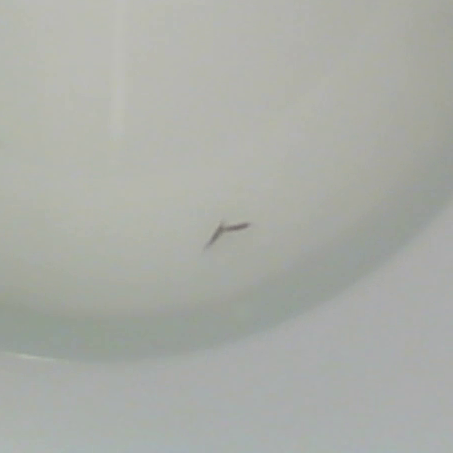
\includegraphics[width=.32\linewidth]{5137}
	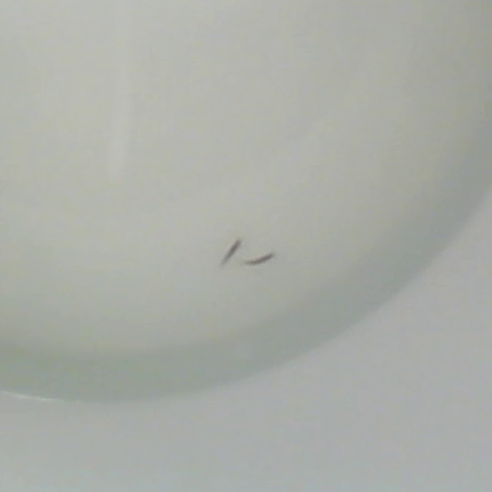
\includegraphics[width=.32\linewidth]{5140}
	\caption{Before and after an overlap}
\end{figure}

However, this method tends to suffer errors in certain scenarios, such as figure~\ref{fig:overlap}, that make an alternative approach needed. When the program tracks the fish, it normally assigns one fish to be red and the other to be blue. Instead what happens here is that the software only returns one fish which it displays as pink. 

\begin{figure}[H]
	\centering
	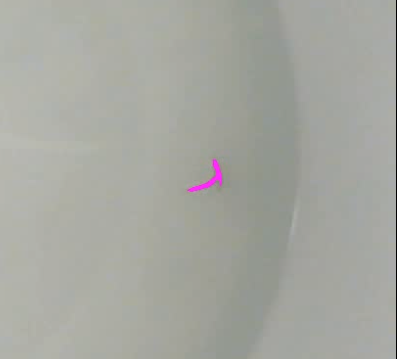
\includegraphics[width=.5\linewidth]{videoScreenshot}
	\caption{An instance where the software can't accurately track the fish}
	\label{fig:overlap}
\end{figure}

The issues can occur in two scenarios, where the fish get close enough that the program returns their only being one fish (figure~\ref{fig:overlap}), and when the fish move fast enough that they are closer to the other's previous position then their previous position. The first of these issues is the easier of the two to check, since it is fairly trivial to check for regions in which only one fish is reported (please see Appendix~\ref{appendix1}). While it is easy enough to check for the first of these issues, the second is a little tougher. To check for errors in these cases, the distance of each fish from its previous position must be compared to the distance from each fish to the other fishes previous position (Appendix~\ref{app:swapStatus}). If the software mistakes the positions of the fish, which we will refer to as a swap, it will look like the fish traveled longer than it should have.

\begin{figure}[H]
	\centering
	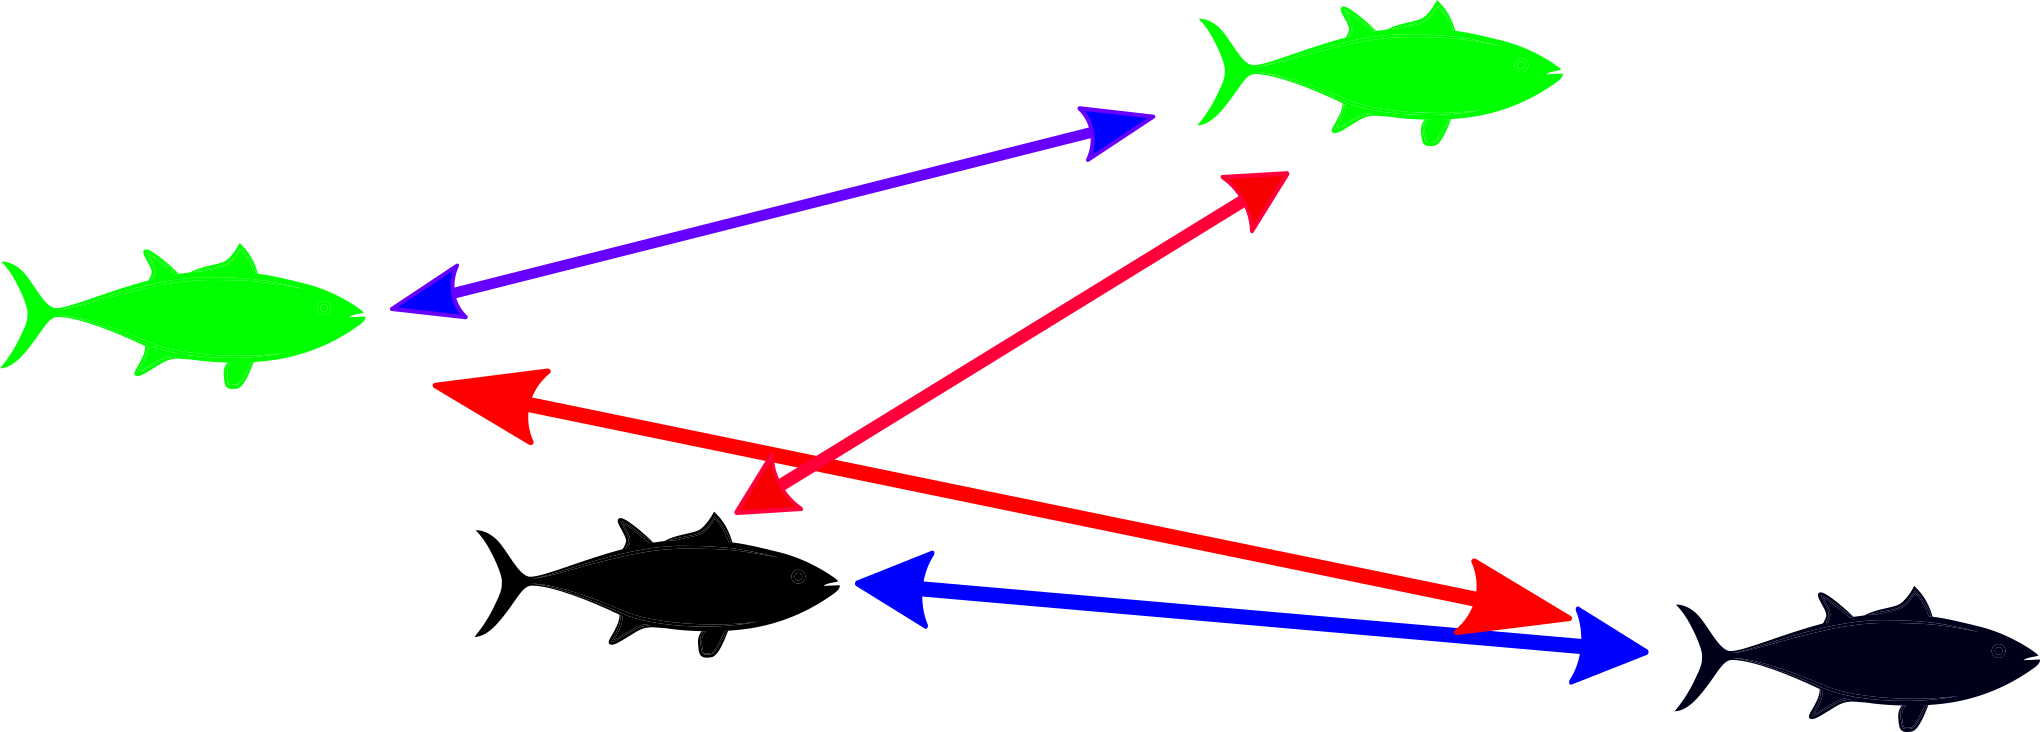
\includegraphics[width=.49\linewidth]{fish3}
	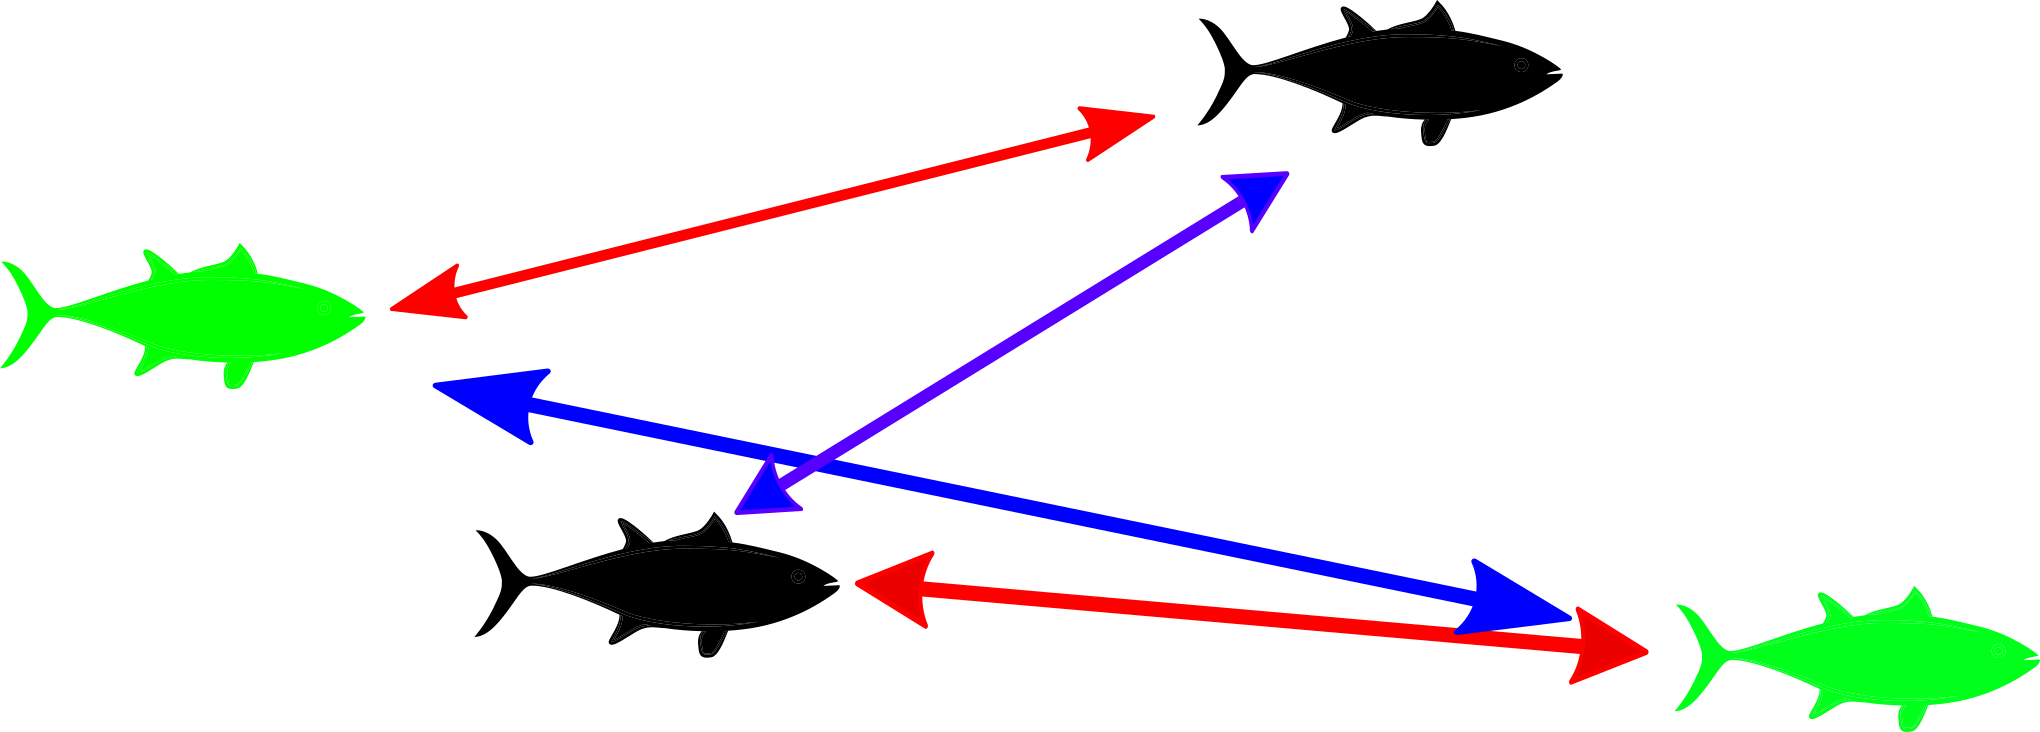
\includegraphics[width=.49\linewidth]{fish4}
	\caption{maintained identities (blue) and swapped identities (red) for two scenarios}
	\label{fig:broverlap}
\end{figure}

What this leads to is issues in the end results, since they are in no way accurate due to this massive source of error. To fix this issue, we are applying two approaches in tandem, both a more common naive technique that tends to fail in areas where the fish are close together but is computationally light and works well when the fish are far apart; and a second one of comparing a unique identifier for each fish from moment to moment to find the fish with the same identifier which is much more accurate, but computationally intensive, which we got from the paper on the idTracker program from when they tried to tackle the same problem\cite{idTracker}. The reason we are using two processes to track the fish is that a common issue of the more common and simpler first method of automatic tracking is that whenever the position of the fish have been confused, the tracker has no way to regain the fishes' position and track which fish is which. To solve this issue, we need a way to track the fish from moment to moment in the cases where this common approach fails, which leads us to the second method.

\subsection{Previous work}
 
%reference idtracker/trex for how to talk about previous works, start broader, start with program that isn't able to auto unswap, recently programs came around that tried to automate this, paragraph about trex?
%\cite all of the papers, cite some of the things that are in the front of the papers, cite papers on mexican cavefish
%several haveemerged recently, all have upsides and downsides, ideal program depends on usecase

Since this is a problem that is common to all animal tracking behaviors, there have been several attempts to provide tracking solutions as alternatives to manual tracking and unswapping. Of these programs that came before, we are basing our work most heavily on a program called idTracker \cite{idTracker}. The authors of that paper also had the problem of there being no existing programs that could either take over the process of fixing the results outputted by a program without any swap correction, or to track the animals with swap correction. Given that the existing technology of the time relied on taking a video of the fish and then having a person manually do error correction, this was non ideal, especially since this approach both had too much error, and that the error tended to compound in on itself over the length of the tracking process. To combat this, the paper proposed a process by which each fish would be given a unique identifier, which the authors decided would be the fishes intensity map, which was created by taking readings of the brightness of the fish and noting unique spots. The process then compares the identifiers frame by frame, to determine which fish is which. We are emulating this process by using a 2d histogram to plot their intensity maps, and using this to compare the frame data.

One thing to note about this process is that it is in no way unique. Since this is a common problem across all biological disciplines that deal with animals on a small scale, multiple solutions have com forth for resolving this issue. Some of the more notable ones are: idTracker.ai, which is an upgrade to the idTracker program using machine learning; trex (cite trex.run), which is another program that using machine learning; and deeplabcut, which also uses machine learning, but is optimized for posture tracking in animals. These programs are in a position where they are adjacent to what the labs we are working with need, they each have pitfalls that make them non ideal. Most prominently, the labs would prefer not to have to train programs to get accurate results, with the biggest offender of this being deeplabcut, in addition to not wanting to deal with the computationally insensitive nature of machine learning. This is in addition to several of the programs giving poor results when used in test cases due to optimization issues, with trex being the worst culprit for this. Instead the decision was made to create a program that was optimized for use by the labs.


\section{Methods}

\subsection{Video Collection}
While any actual experimentation on the fish is beyond the scope of this thesis, it is still useful to describe the process of gathering data. The basic setup of the labs we are taking data from is a tank with two fishes in it and a camera trained on them, as seen below.

\begin{figure}[H]
	\centering
	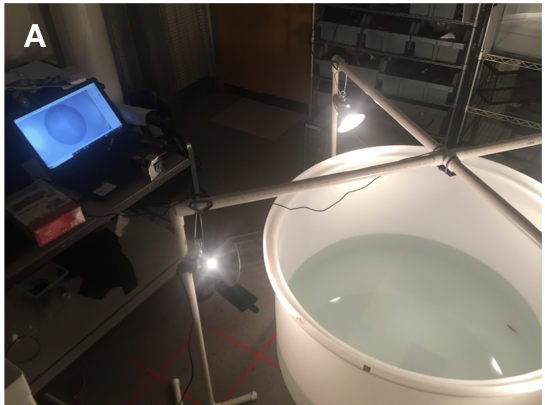
\includegraphics[width=.5\linewidth]{experimental_design}
	\caption{The tank setup}
\end{figure}

This setup produces a video for us to use, of which an example frame is shown below.

\begin{figure}[H]
	\centering
	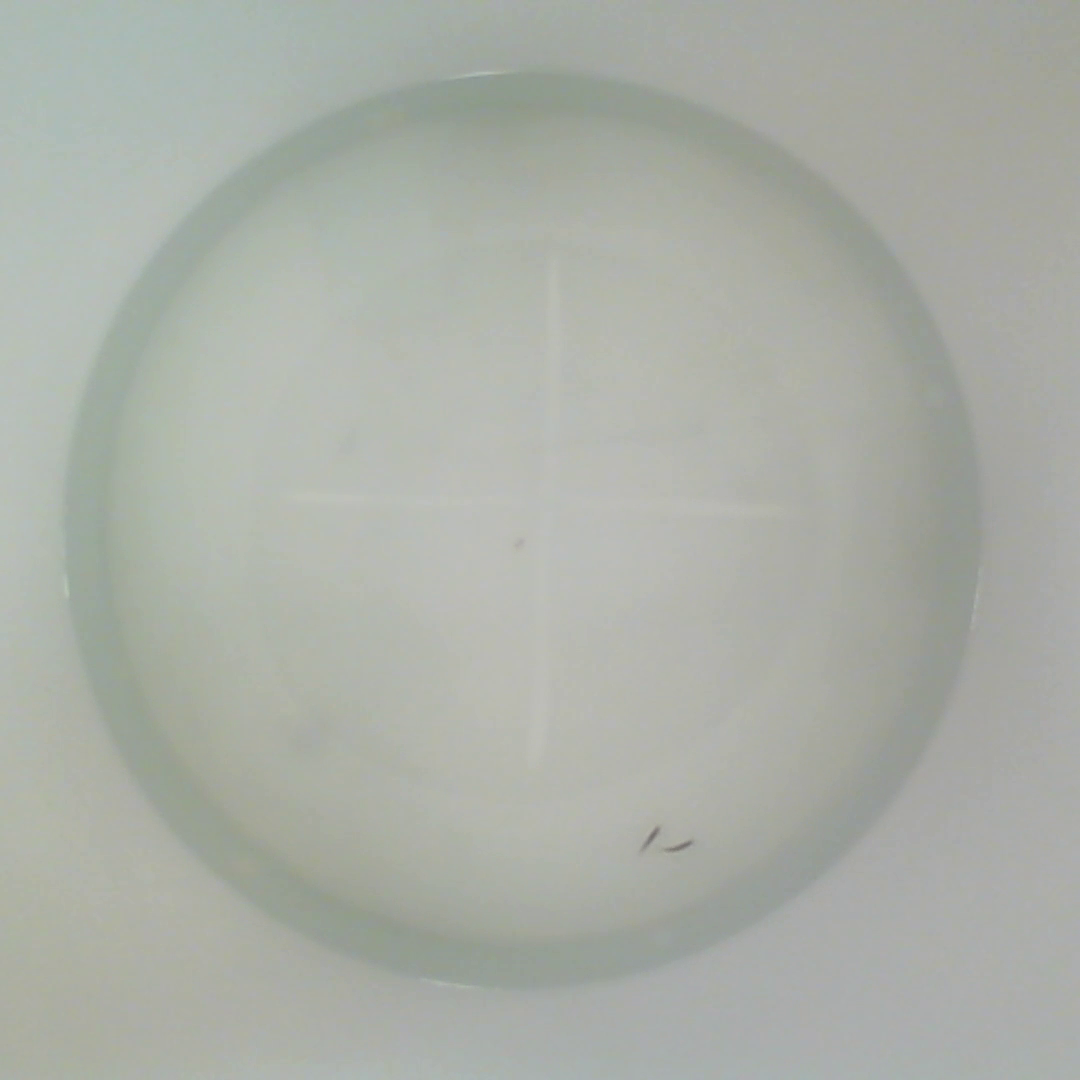
\includegraphics[width=.5\linewidth]{figures.frame5140}
	\caption{An example frame of the video}
\end{figure}

\subsection{Current Tracking}
%following is over explained
%say focusing on two fish somewhere
%expand this section

To track the fish, we must first feed the video captured from this setup to an analysis program, in our case cdtracker (cite https://github.com/yffily/trilab-tracker), which has been especially created for use by the Jupiter Trilab. This program takes the tank as a preseet constant background, and The

The tracker works taking the tank as a constant background, and noting that the fish are the only dark spots on the tank. It then returns an array for each of the fish containing a list of the fish's pixels and those pixel's colors. Once we have the fish saved in a format that we can analyze, we are ready to start working on the tracking of the fish. Since each the way we store the data gives each fish an identifier, we then can use those identifiers to analyse the fish.

The next step is to segment the data into regions based on the number of fish it detects. We do this because the distance based unswapping approach doesn't work on regions where there is only one fish detected, so we need to tell the program where it can use that approach.

\begin{figure}[H]
	\centering
	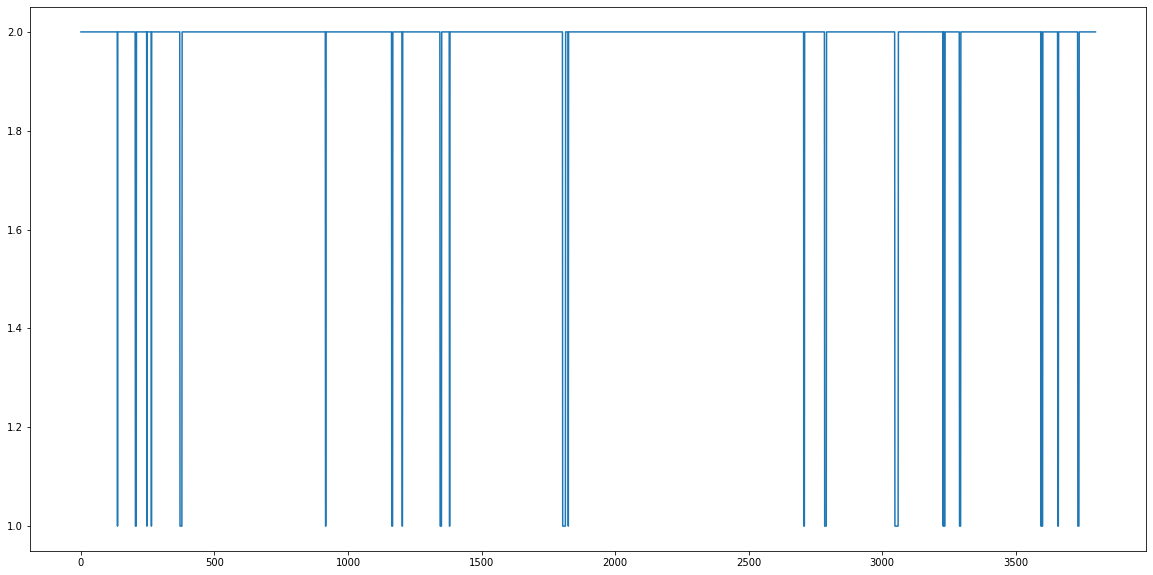
\includegraphics[width=.75\linewidth]{oneFish}
	\caption{Number of one fish regions}
\end{figure}


\subsection{Distance Based Unswapping}
\begin{figure}[H]
	\centering
	\includegraphics[width=.75\linewidth]{fish2}
	\caption{Basic overview of unswapping logic}
\end{figure}
%remove matrix, talk about comparing distance traveled/be more specific in labels.
%put more stuff in here. use more figures, show graphs of number of swaps before and after

The default method that the program uses to determine which fish is which is to assume that the fish closest to their previous positions are the same fish. However, this tends to fail in areas in which either the fish have moved a great distance since the last frame, or the case in which the fish are close enough that the program returns their only being one fish, in which case the program will basically assume which fish is which at random. To combat this we will use several methods. The first of these is distance based unswapping, which works by 

The first approach we tried is taking the positions of the fish and comparing how close they were to their previous positions to check for swaps. This approach works on the regions where there are two fish detected (``nonoverlapping range''), and so we need to confine it to those regions. 

\subsection{Histogram Based Unswapping}
In the overlapping (or regions where one fish is detected), we need an identifier for the fish, so we will use bright spots on fish as this identifier. Once we have those identifiers, the easiest way to compare these identifiers is to create histogram of the brightness of the fish. We can then have the program compare the slight differences, because even though look same, they are different enough that the code can pick up the differences. However, one issue that we ran into is that the fish we are using are subpar because they are too uniform in brightness.

%talk about euclidian distance

\begin{figure}[H]
	\centering
	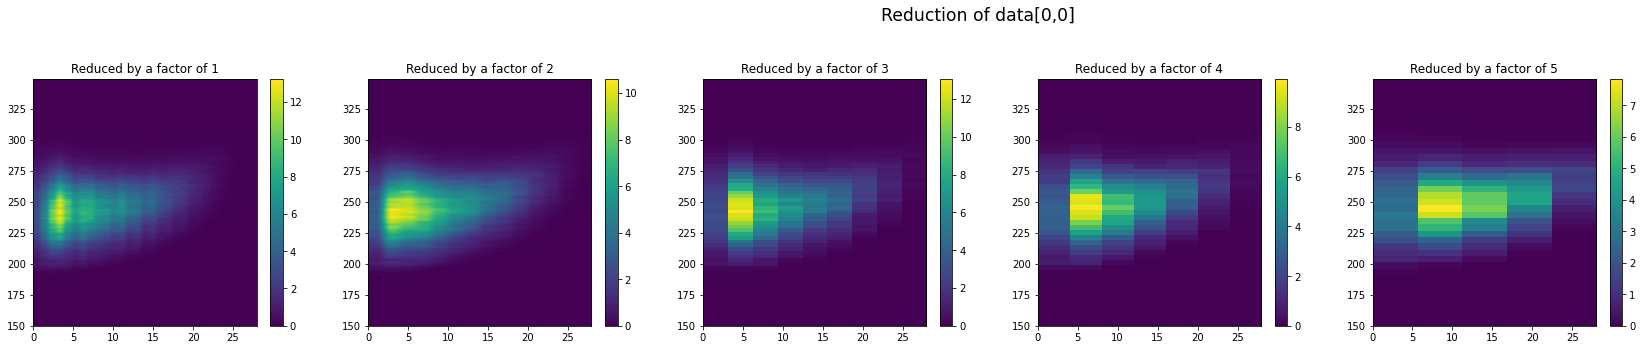
\includegraphics[width=\linewidth]{reducedHist}
	\caption{The histograms}
	\label{fig:reducedHist}
\end{figure}


\section{Results}

\subsection{Accuracy}
%\textbf{\textit{show pictures and describe accuracy.}}

Without any tuning, the accuracy rate is only 19\%. This is probably due to the fish being too uniform, as once are able to tune the process, we can expect a slightly more accurate result.

\begin{figure}[H]
	\centering
	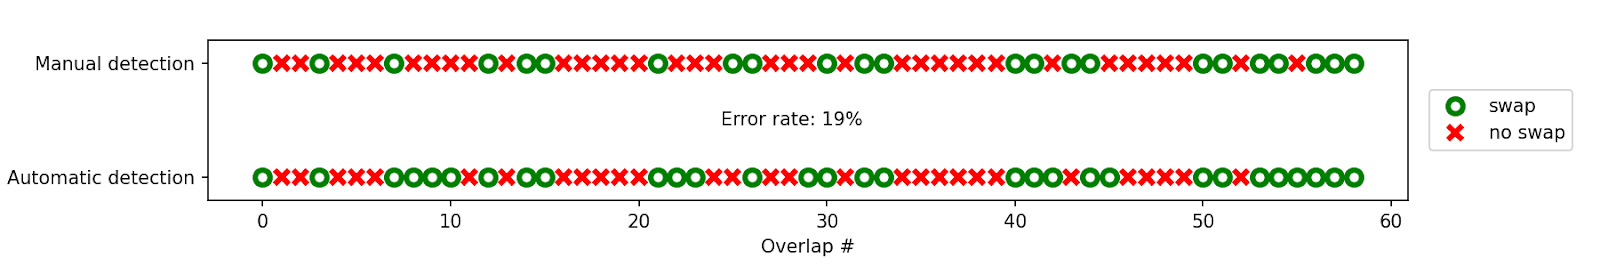
\includegraphics[width=\linewidth]{error}
	\caption{The error of the untuned process}
\end{figure}

\subsection{Bin Reduction}

One thing that was also tested was what would happen if we used less bins on teh histograms that we used for analysis, both to see how it affected accuracy and performance. What was found was that there was no significant change in the accuracy of the data when this opperation was performed.

\section{Code?}

Once we have this data for the nonoverlapping ranges, we have to switch approaches for the overlapping regions. Since we can't compare the distances with the software only reporting a single fish, we are forced to use a different technique., we are using the technique of comparing the histograms of the brightness of the fishes before and after an overlapping range, as proposed by the paper on idTracker\cite{idTracker}. The process for this is for us to feed the arrays directly into numpy's histogram2d, which allows us to compute the histograms with a minimal amount of effort other than determining the correct bins. After that we need to manipulate the data slightly so that the histograms are taken as the average over the nonoverlapping regions for more accuracy, and are then saved out for comparison.

We can then feed this representation into a simple value comparison to check for swaps. When rendered to a more human readable form, we can either get a list of frames, or a graphs as shown below.

\begin{figure}[H]
	\centering
	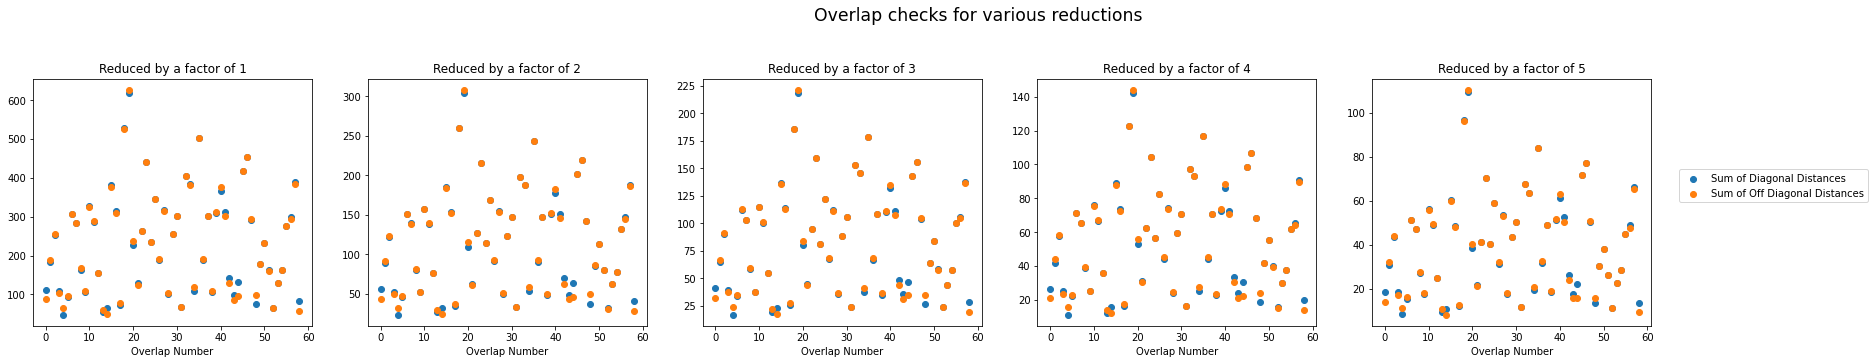
\includegraphics[width=\linewidth]{reducedGraph}
	\caption{The graphs from the histograms}
	\label{fig:reducedGraph}
\end{figure}


\appendix
\section{Appendix A}
\label{appendix1}

\begin{minipage}[c]{\textwidth}
\begin{lstlisting}[language=Python]
i2=0
nonOverlappingRange=[]
while i2<len(fish):
    i1=i2
    while i1<len(fish) and len(fish[i1])!=2:
        i1+=1
    i2=i1
    while i2 < len(fish) and len(fish[i2])==2:
        #find the first overlapping index
        i2+=1
    nonOverlappingRange.append([i1,i2])
print(nonOverlappingRange)
\end{lstlisting}
\end{minipage}

\section{Appendix B}
\label{app:swapStatus}

\begin{minipage}[c]{\textwidth}
\begin{lstlisting}[language=Python]
def swapStatus(pos,i):
    '''
    Detect swaps between consecutive frames based on proximity.
    
    Input:
        pos:Postionts. Array with shape (Nframes,Nfish,Ndimensions),
        i: Frame index. Int.
    
    Output:
        Int. 0 if no swaps, 1 if swapped, 2 if overlapping.
    '''
    nFish=pos.shape[1] #Number of fish
    distanceMatrix=[np.linalg.norm(pos[i+1][0]-pos[i][0]),
                    np.linalg.norm(pos[i+1][1]-pos[i][1]),
                    np.linalg.norm(pos[i+1][0]-pos[i][1]),
                    np.linalg.norm(pos[i+1][1]-pos[i][0])]
    swapCriteron=(distanceMatrix[0]+distanceMatrix[1])-(distanceMatrix[2]+distanceMatrix[3])
    if abs(swapCriteron)<1e-10:
        return 2 #Overlapping
    elif swapCriteron>0:
        return 1 #Swapped
    elif swapCriteron<0:
        return 0 #Normal
    else:
        return -1
\end{lstlisting}
\end{minipage}

\section{Appendix C}
\label{app:dataShape}

The data is stored in an array of shape [frame][fish][xpixels,ypixels][color]

\textit{\textbf{Picture Here}}

\section{Appendix D}
\label{app:histCreator}

\begin{minipage}[c]{\textwidth}
\begin{lstlisting}[language=Python]
for i in tnrange(60,desc='nonOverlappingRange'):
    for k in range(2):
        countSum=0
        countDif=0
        pairData=[]
        for j in range(*nonOverlappingRange[i]):
            fishPixels = fishU[j][k]
            m,l=np.triu_indices(fishPixels.shape[0],k=1)
            d=np.sqrt((fishPixels[l,0]-fishPixels[m,0])**2+(fishPixels[l,1]-fishPixels[m,1])**2)
            bSum=fishPixels[l,2]+fishPixels[m,2]
            bDif=fishPixels[l,2]-fishPixels[m,2]

            heightValuesSum,_,_=np.histogram2d(d,bSum,bins=(binsDist,binsSum))
            histSum+=heightValuesSum
            countSum+=1
            heightValuesDif,_,_=np.histogram2d(d,bDif,bins=(binsDist,binsDif))
            histDif+=heightValuesDif
            countDif+=1
        histSum/=countSum
        histSumList[i,k]=histSum.copy()
        histDif/=countDif
        histDifList[i,k]=histDif.copy()
\end{lstlisting}
\end{minipage}

%==========================================================================
% Bibliography.

%\printbibliography
%\bibliographystyle{plain}
%\bibliography{fish}


\end{document}
